% =========================
% CHƯƠNG 14
% =========================
\chapter{Trực quan hóa và giám sát}

\section{Bảng điều khiển thời gian thực}

Trực quan hóa và giám sát là thành phần quan trọng giúp theo dõi hiệu quả vận hành, hỗ trợ phân tích và tối ưu hệ thống. Bảng điều khiển (dashboard) cho phép người dùng quan sát trạng thái giao thông, pha đèn tín hiệu, hàng chờ, tốc độ, thời gian chờ, cùng các sự kiện đặc biệt như ưu tiên xe khẩn cấp hoặc tắc nghẽn.

\subsection{Kiến trúc và chức năng chính}
Dashboard được phát triển bằng Python (tkinter + matplotlib), tích hợp trực tiếp với bộ điều khiển giao thông. Dữ liệu được cập nhật liên tục, hiển thị các thông số quan trọng như trạng thái pha, hàng chờ, thời gian chờ, tốc độ trung bình trên từng làn.

\begin{figure}[H]
    \centering
    \fbox{%
        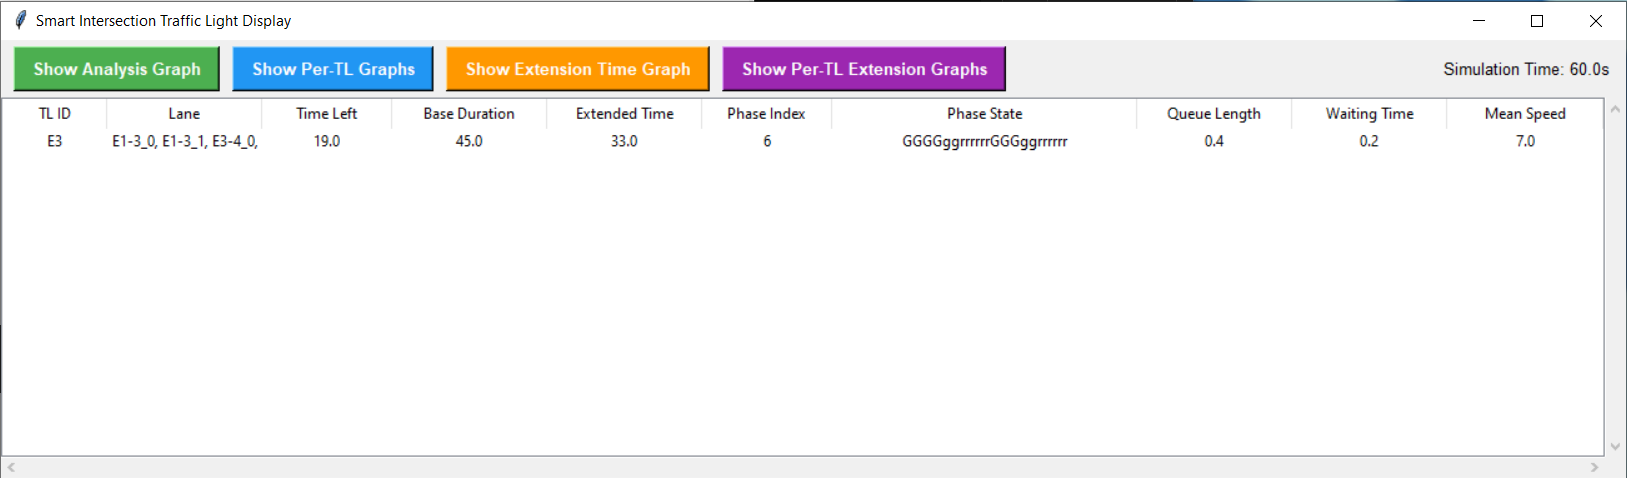
\includegraphics[width=0.95\textwidth]{image1.png}
    }
    \caption{Giao diện bảng điều khiển SmartIntersectionTrafficDisplay}
    \label{fig:dashboard_gui}
\end{figure}

\subsection{Các nhóm chức năng}
\begin{itemize}
    \item \textbf{Theo dõi trạng thái pha}: Hiển thị thời gian còn lại, duration cơ bản, extended time, trạng thái hiện tại của từng pha.
    \item \textbf{Giám sát hàng chờ và tốc độ}: Biểu đồ hàng chờ, thời gian chờ, tốc độ trung bình từng làn.
    \item \textbf{Trực quan hóa lịch sử điều chỉnh}: Thống kê các lần điều chỉnh duration, extended time, so sánh với baseline.
    \item \textbf{Hiển thị sự kiện đặc biệt}: Cảnh báo các sự kiện như ưu tiên xe khẩn cấp, rẽ trái bảo vệ, tắc nghẽn.
\end{itemize}

\subsection{Luồng dữ liệu}
Dashboard truy xuất dữ liệu từ controller qua API, cập nhật dữ liệu mỗi giây. Các chỉ số hiệu năng, sự kiện và trạng thái hệ thống được lưu lại phục vụ phân tích hậu kỳ.

\section{Phân tích dữ liệu hậu kỳ}

Dữ liệu sự kiện và trạng thái từ dashboard được lưu trữ để phục vụ phân tích offline. Các chức năng chính gồm:
\begin{itemize}
    \item Phân tích pattern điều chỉnh pha và extended time.
    \item Thống kê thời gian chờ trung bình, độ dài hàng chờ, số lần congestion/starvation.
    \item So sánh hiệu năng giữa các nút giao hoặc nhóm cluster.
\end{itemize}

\begin{lstlisting}[style=py,caption={Ví dụ: Thống kê thời gian chờ trung bình}]
import pandas as pd
def compute_average_wait_time(phase_events):
    df = pd.DataFrame(phase_events)
    avg_wait = df.groupby("phase_idx")["duration"].mean()
    print("Thoi gian cho trung binh theo pha:")
    print(avg_wait)
\end{lstlisting}

\section{Đồng bộ và mở rộng}

\begin{itemize}
    \item Dữ liệu dashboard được đồng bộ lên Supabase để phục vụ giám sát từ xa và phân tích tổng hợp.
    \item Có thể mở rộng dashboard với các công cụ hiện đại (plotly, dash), hỗ trợ phân tích động, replay video, kết nối cảm biến thực tế.
\end{itemize}
